\section{Question}

\subsection{Translate your cDNA sequence into protein/amino acid sequence. How many amino acids does your protein contain?  }

The translation of the \textit{cDNA} contains \textbf{3143} amino acids, which makes sense given the \textit{Coding Sequence} is \textbf{9429} nucleotides long:

\[
    9429 / 3 = 3143
\]

\medskip

% - - - - - - - - - - - - - - - - - - - - - - - - - - -

\subsection{Of the 64 possible codons available, how many are used?}

Out of the 64 possible codons available, \textbf{62} codons are used. \textbf{UAA} and \textbf{UAG} are not used.

\medskip

% - - - - - - - - - - - - - - - - - - - - - - - - - - -

\subsection{What is the most common amino acid in the protein?}

The most common amino acid in the \textit{huntingtin} protein is \textbf{Leucine} \textit{(Leu/L)} - see figure \ref{fig:amino-acids-hist}.

\begin{figure}[ht]
    \centering
    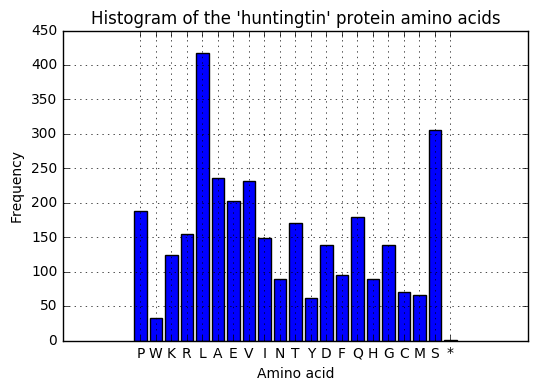
\includegraphics[width=0.8\linewidth]{res/amino-acids-hist.png}
    \caption{Histogram obtained with the Jupyter Notebook.}
    \label{fig:amino-acids-hist}
\end{figure}

\medskip

% - - - - - - - - - - - - - - - - - - - - - - - - - - -

\subsection{How many codons for this amino acid exist and how often is each used?}

\textit{Leucine} has 6 coding amino acids. Below is a table with their respective frequencies in the \textit{huntingtin} protein.

\bigskip

\begin{center}
	\begin{tabu} to 0.4\textwidth{ | X[c] | X[c] | }
		\hline
		Codon & Frequency \\
		\hline
		UUA & 70 \\
		UUG & 156 \\
		CUU & 168 \\
		CUC & 178 \\
		CUA & 68 \\
		CUG & 295 \\
		\hline
	\end{tabu}
\end{center}

\clearpage

\newpage
